\chapter{Contribuciones de código abierto}\label{annex:contributions}

% # Code to convert URLs to the commands above
%
% import re
% import fileinput
% from github import Github
%
% URL_REGEX = r'https?://github\.com/([\w_-]+/[\w_-]+)/(\w+)/(\d+)'
% AUTH = 'OMITTED'
%
%
% def get_kind(base: str, state: str) -> str:
%     if base == 'pull':
%         return 'pr'
%     else:
%         return 'issue'
%
%
% g = Github(AUTH)
%
% for url in fileinput.input():
%     matches = re.search(URL_REGEX, url)
%     if matches is None:
%         print(f"`{url}` isn't an URL, skipping...")
%         continue
%
%     repo_name = matches.group(1)
%     kind_base = matches.group(2)
%     number = int(matches.group(3))
%
%     repo = g.get_repo(repo_name)
%     issue = repo.get_issue(number=number)
%     kind = get_kind(kind_base, issue.state)


% Custom command for easy issue/pr formatting
\newcommand{\issue} {\begingroup
    \catcode`_=12 \github{issues}{Imagenes/issue.pdf}}
\newcommand{\pr} {\begingroup
    \catcode`_=12 \github{pull}{Imagenes/pr.pdf}}
\newcommand{\github}[5] {%
    \item \includegraphics{#2} \; \emph{#5}\\
        \href{https://github.com/#3/#1/#4}{\texttt{github.com/#3/#1/#4}}
    \endgroup
}

Una de mis partes favoritas del proyecto ha sido poder contribuir tanto a
diferentes dependencias de código abierto, así que he mantenido una lista de
todas las ocurrencias. Algunas colaboraciones son más importantes que otras,
pero sigue siendo una buena métrica de los resultados obtenidos. Esto no incluye
aquellos issues o pull requests que:

\begin{itemize}
    \item No contribuyeron nada (por ejemplo, preguntas o ideas descartadas).

    \item Fueron repetitivos (por ejemplo, tuve que realizar varios pull
        requests idénticos en Tremor para lidiar con problemas con Git).

\end{itemize}

\section{Contribuciones externas}

En esta sección se incluyen todas aquellas contribuciones a repositorios que no
tengan relación directa con Tremor.

\begin{enumerate}
    \issue{rust-lang/nomicon}{338}{Subtyping and Variance --- Trait variance not covered}

    \issue{szymonwieloch/rust-dlopen}{42}{\code{dlerror} *is* thread-safe on some platforms}

    \issue{wasmerio/wasmer}{2539}{Add deprecation notice to the crate \code{wasmer-runtime}}

    \pr{oxalica/async-ffi}{10}{Support for \abistable}

    \pr{oxalica/async-ffi}{11}{Cbindgen support}

    \issue{oxalica/async-ffi}{12}{Procedural macro for boilerplate}

    \issue{rodrimati1992/abi_stable_crates}{52}{Generating C bindings}

    \pr{rodrimati1992/abi_stable_crates}{55}{Fix `carte' typo}

    \pr{rodrimati1992/abi_stable_crates}{57}{Fix some more typos}

    \pr{rodrimati1992/abi_stable_crates}{58}{Add support for \code{.keys()} and \code{.values()} in RHashMap}

    \pr{rodrimati1992/abi_stable_crates}{59}{Implement \code{Index} for slices and vectors}

    \issue{rodrimati1992/abi_stable_crates}{60}{Stable ABI for floating point numbers}

    \pr{rodrimati1992/abi_stable_crates}{61}{Support for \code{f32} and \code{f64}}

    \pr{rodrimati1992/abi_stable_crates}{68}{Implement \code{ROption::as_deref}}

    \pr{rodrimati1992/abi_stable_crates}{70}{Implement \code{RVec::append}}

    \pr{rodrimati1992/abi_stable_crates}{76}{Fix \code{R*} lifetimes}

    \pr{rodrimati1992/abi_stable_crates}{77}{Fix inconsistencies with \code{RVec} in respect to \code{Vec}}

    \pr{rodrimati1992/abi_stable_crates}{82}{Implement \code{ROption::{ok_or,ok_or_else}}}

    \pr{rodrimati1992/abi_stable_crates}{83}{\code{RHashMap::raw_entry[_mut]} support}

    \pr{rodrimati1992/abi_stable_crates}{85}{Fix hasher}

    \pr{rodrimati1992/abi_stable_crates}{88}{Only implement \code{Default} once}

    \pr{simd-lite/simd-json-derive}{9}{Support for \abistable}

    \issue{simd-lite/simd-json-derive}{10}{No docs for v0.3.0}

    \pr{simd-lite/value-trait}{14}{Add support for StableAbi}

    \pr{simd-lite/value-trait}{16}{User friendliness for the win! (close \#15)}

    \pr{simd-lite/value-trait}{18}{Update \abistable after upstreamed changes}

    \pr{nagisa/rust_libloading}{94}{Small typo}

    \pr{szymonwieloch/rust-dlopen}{40}{Fix typo}

    \pr{Licenser/halfbrown}{13}{Implement \code{remove_entry}}

    \pr{Licenser/halfbrown}{14}{Implement \code{Clone} and \code{Debug} for \code{Iter}}

    \pr{Licenser/halfbrown}{16}{Relax constraints}

    \pr{Licenser/halfbrown}{17}{Same \code{Default} constraints}

    \pr{Licenser/halfbrown}{18}{Fix \code{Clone} requirements for \code{Iter}}

\end{enumerate}

\section{Contribuciones internas}

Esta sección lista los pull requests o issues realizadas dentro de los
repositorios de Tremor, tanto para el sistema de plugins, como para otras
mejoras no relacionadas.

\begin{enumerate}
    \pr{tremor-rs/tremor-runtime}{1434}{PDK support}

    \pr{marioortizmanero/tremor-runtime}{11}{PDK with a single value}

    \pr{tremor-rs/tremor-runtime}{1447}{Fix \code{makefile bench}}

    \pr{marioortizmanero/tremor-runtime}{2}{Adding \abistable support for \code{tremor-script}}

    \pr{marioortizmanero/tremor-runtime}{1}{Adding \abistable support for \code{tremor-runtime}}

    \pr{tremor-rs/tremor-runtime}{1303}{Adding \abistable support for \code{tremor-value}}

    \pr{tremor-rs/tremor-runtime}{1287}{Plugin Development Kit: Connectors}

    \issue{tremor-rs/tremor-runtime}{1353}{\code{deny} statemements in \code{lib.rs} should be enforced in the CI rather than in the code}

    \pr{tremor-rs/tremor-www}{72}{Fix wrong links in getting started}

    \issue{tremor-rs/tremor-www}{73}{Redirect \code{docs.tremor.rs} to \code{www.tremor.rs/docs}}

    \pr{tremor-rs/tremor-www}{186}{Links pinned to 0.12 don't work}

    \pr{tremor-rs/tremor-www}{187}{Small fix in code snippet}

    \issue{tremor-rs/tremor-www}{195}{No margins in benchmark page}

\end{enumerate}

\section{Otras contribuciones}

Otro logro del que me siento extrañamente orgulloso es de accidentalmente romper
el mismo compilador de Rust, como se ve en la Figura~\ref{fig:rustc_crash}. El
error ya había sido reportado hace unos meses, pero los intentos de arreglarlo
parecían haber fallado, así que dejé un comentario indicando cómo me había
ocurrido a mí. Debería estar arreglado en la siguiente versión del compilador, y
no me ha vuelto a ocurrir desde entonces~\cite{rustc_fix}

\begin{figure}[H]
    \centering
    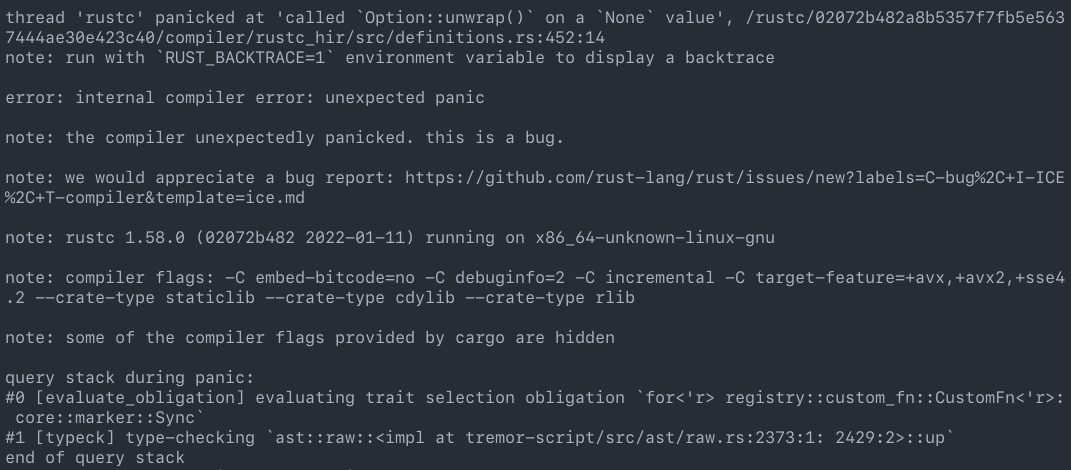
\includegraphics[width=\textwidth]{./Imagenes/rustc_crash.png}
    \caption{Error de compilación de \code{rustc}, relacionado con la
    compilación incremental y arreglado ya en una futura
    versión.}%
    \label{fig:rustc_crash}
\end{figure}

Adicionalmente, el programa \emph{LFX Mentorship} finaliza con un evento en
enero en el que los participantes que quieran pueden mostrar su trabajo una vez
terminado~\cite{lfx_showcase}. Consiste en realizar una presentación de 15
minutos en la que explican su experiencia, lo cual es especialmente útil para
aquellos que quieran unirse al programa en el futuro. No es lo suficientemente
larga como para entrar en detalles de implementación, lo que la hace una buena
introducción al proyecto: \url{https://youtu.be/htLCyqY0kt0?t=3166}.
